\documentclass{article}

\usepackage{amsmath}
\usepackage{listings}
\usepackage{color}
\usepackage{sectsty}
\usepackage{spverbatim}
\usepackage{titlesec}
\usepackage{graphicx}
\usepackage{hyperref}

\graphicspath{ {./images/} }

\definecolor{dkgreen}{rgb}{0,0.6,0}
\definecolor{gray}{rgb}{0.5,0.5,0.5}
\definecolor{mauve}{rgb}{0.58,0,0.82}

\lstset{frame=tb,
  language=Java,
  aboveskip=3mm,
  belowskip=3mm,
  showstringspaces=false,
  columns=flexible,
  basicstyle={\small\ttfamily},
  numbers=none,
  numberstyle=\tiny\color{gray},
  keywordstyle=\color{blue},
  commentstyle=\color{dkgreen},
  stringstyle=\color{mauve},
  breaklines=true,
  breakatwhitespace=true,
  tabsize=3
}

\sectionfont{\fontsize{10}{13}\selectfont}
\titlespacing*{\section}{0pt}{0.3\baselineskip}{0.3\baselineskip}
\title{Project 2: Docker}
\author{Jonathan Carona}
\date{\today}
\begin{document}
\section{Prerequisites and experiment setup}
The system this project is running on is on PopOS 22.04 LTS which is
based on Ubuntu 22.04 LTS. In Project 1, I chose to investigate and optimize the learning rate,
train batch size and optimizer type hyperparameters, the optimal values that were found were
6.991860954982597e-05, 256, Adam respectively.

\section{Task 1: Migrate Notebook to Python Scripts}
The Python Notebook was migrated into a single Python script. This script can receive arguments upon running the script like so:

\verb!python distilbert_on_mrpc.py --learning_rate 1e-05!

The arguments are parsed with 'argparse' and added to the model. If a specific or no arguments were passed, then it uses the default values.
\begin{lstlisting}
    import argparse
    parser = argparse.ArgumentParser()
    parser.add_argument('--learning_rate', dest='learning_rate', type=float)
    parser.add_argument('--adam_epsilon', dest='adam_epsilon', type=float)
    ...
    \end{lstlisting}

The experiments are logged using wandb.ai.

\section{Task 2: Creating a Docker Image}
The created docker image contains the python script and installs all libraries from the requirements.txt file.
When running the container, just like in task 1, the hyperparameters can be passed as arguments. 
The following command runs a single training run with the best parameters:

\begin{spverbatim}
    sudo docker run run_distilbert_training python3 ./distilbert_on_mrpc.py --api_key YOUR_WANDB_API_KEY --learning_rate 6.991860954982597e-05 --train_batch_size 256 --optimizer_type Adam    
    \end{spverbatim}

NOTE: The wandb api key is a parameter here. I am aware that this does not follow standards. In a company setting, the key would be in a safe place and retrieved from there. But just for the sake of this school project, it makes it easier to test for other students.


This is how the docker image is installed and structured:

\begin{lstlisting}
    # syntax=docker/dockerfile:1
    FROM python:3.10-slim
    WORKDIR /usr/app/src
    COPY ./distilbert_on_mrpc.py ./ 
    COPY ./requirements.txt ./ 
    RUN pip install --no-cache-dir -r requirements.txt
    CMD ["python3", "./distilbert_on_mrpc.py"]
    \end{lstlisting}
... by running the command: 
\verb!sudo docker build -t run_distilbert_training .!

\section{Task 3: Running the Docker Image on Playground}
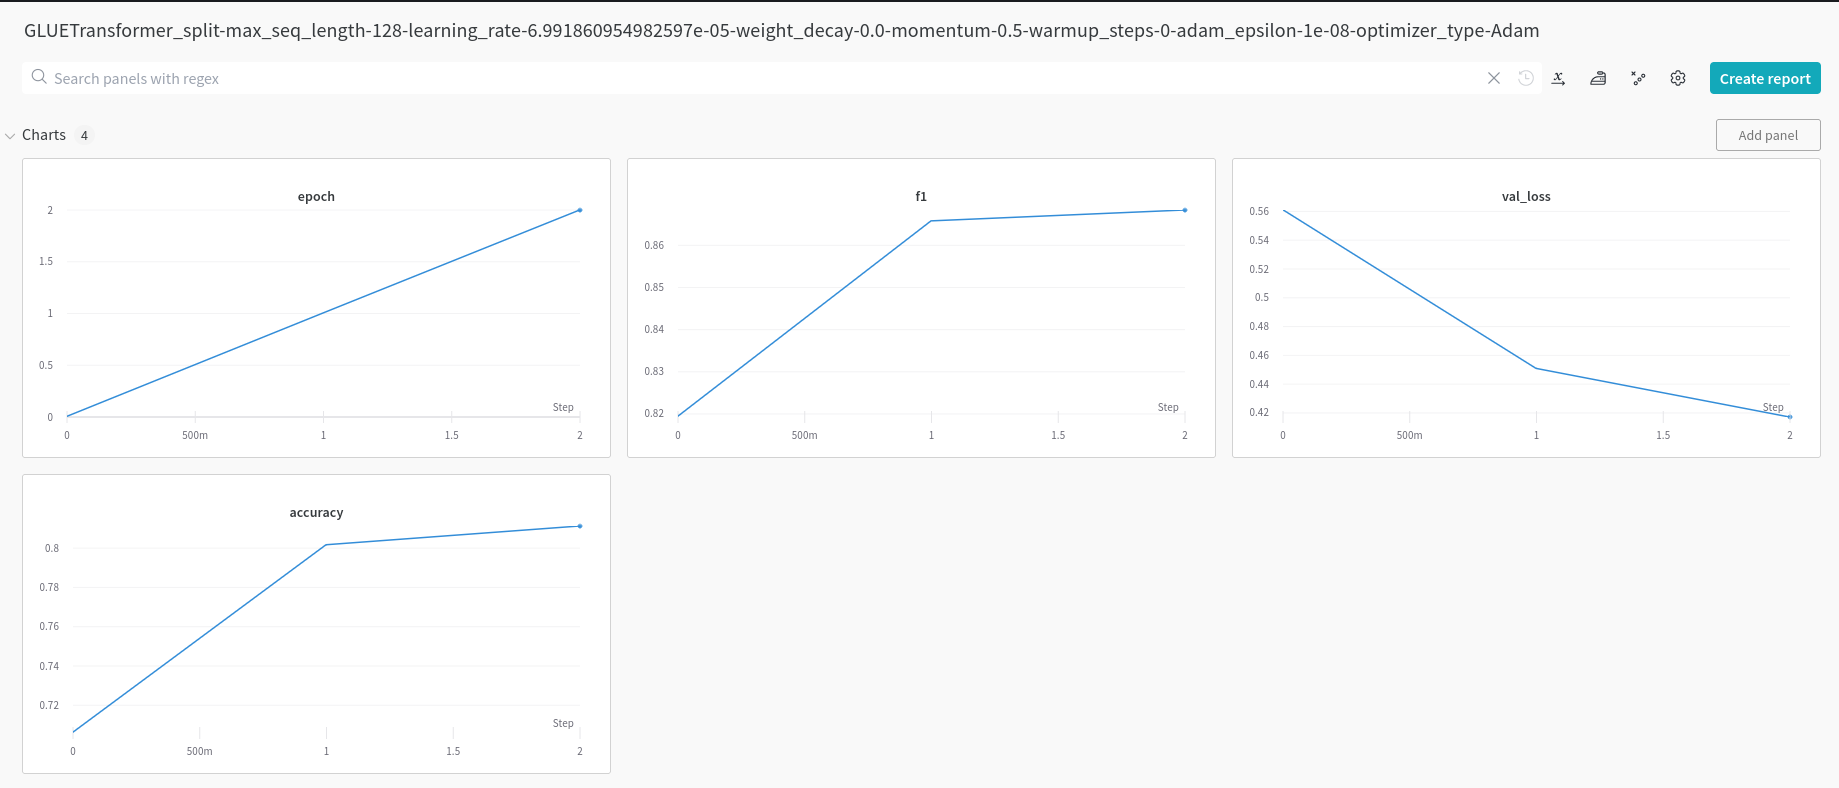
\includegraphics[width=5cm, height=4cm]{local}

\section{Task 4: Setup GitHub Repository}
Below is a link to my private project. You can find additional information and help under the readme section.


\href{https://github.com/JDCarona/project2-mlops}{GitHub Project 2}.




\section{Reflection}
It took for me a lot of time to setup the docker image file for it to be able to take in hyperparameter arguments.
I have never worked with docker before, so I expected this. 

What 


\end{document}